\section{Matrix Norms and the Condition Number}

\begin{bigidea}
Given a linear system $A \bs{x} = \bs{b}$, the condition number of $A$ quantifies how sensitive the solution $\bs{x}$ is relative to perturbations in $\bs{b}$.
\end{bigidea}

\begin{definition}
A {\bf norm} on $\mathbb{R}^n$ \cite[p.53]{MH} is a function $\| \cdot \|$ such that:
\begin{enumerate}
\item $\| \bs{x} \| \geq 0$ for all $\bs{x} \in \mathbb{R}^n$
\item $\| \bs{x} \| = 0$ if and only if $\bs{x} = \bs{0}$
\item $\| c \bs{x} \| = |c| \| \bs{x} \|$ for any $c \in \mathbb{R}$ and $\bs{x} \in \mathbb{R}^n$
\item $\| \bs{x} + \bs{y} \| \leq \| \bs{x} \| + \| \bs{y} \|$ for all $\bs{x} , \bs{y} \in \mathbb{R}^n$ (the {\bf triangle inequality})
\end{enumerate}
\end{definition}

\begin{example} Let $\bs{x} = [x_1 \ \cdots \ x_n ]^T \in \mathbb{R}^n$.
\begin{enumerate}
\item The 2-norm is given by the familiar formula
$$
\| \bs{x} \|_2 = \sqrt{ | x_1|^2 + \cdots + | x_n |^2 } = \sqrt{ \sum_{k=1}^n | x_k |^2 }
$$
\item More generally, the $p$-norm is given by
$$
\| \bs{x} \|_p = \left( \sum_{k=1}^n | x_k |^p \right)^{1/p}
$$
For example, a commonly used norm is the 1-norm
$$
\| \bs{x} \|_1 =  | x_1| + \cdots + | x_n | = \sum_{k=1}^n | x_k |
$$
\item The $\infty$-norm is given by
$$
\| \bs{x} \|_{\infty} = \max_k | x_k |
$$
\end{enumerate}
\end{example}

\begin{example} \phantom{.}
\begin{enumerate}
\item Prove that the $\infty$-norm satisfies the required properties of a norm.
\item Sketch the ``unit ball" in $\mathbb{R}^2$ for each norm:
\begin{align*}
B_1 &= \{ \mathbf{x} \in \mathbb{R}^2 : \| \bs{x} \|_1 = 1 \} \\
B_2 &= \{ \mathbf{x} \in \mathbb{R}^2 : \| \bs{x} \|_2 = 1 \} \\
B_{\infty} &= \{ \mathbf{x} \in \mathbb{R}^2 : \| \bs{x} \|_{\infty} = 1 \}
\end{align*}
\item Which set of inequalities is always true? Explain.
$$
\| \bs{x} \|_1 \leq \| \bs{x} \|_2 \leq \| \bs{x} \|_{\infty}
\hspace{5mm} \text{or} \hspace{5mm}
\| \bs{x} \|_1 \geq \| \bs{x} \|_2 \geq \| \bs{x} \|_{\infty}
$$
\end{enumerate}
\end{example}

\begin{definition}
Choose a vector norm $\| \cdot \|$. The corresponding {\bf matrix norm} (or {\bf operator norm}) \cite[p.54]{MH} is
$$
\| A \| = \max_{\bs{x} \not= \bs{0} } \frac{\| A \bs{x} \|}{ \| \bs{x}  \|}
$$
Note that $\| A \bs{x} \| / \| \bs{x} \|= \| A ( \bs{x} / \| \bs{x} \| ) \|$ therefore
$$
\| A \| = \max_{ \| \bs{x} \| = 1 } \| A \bs{x} \|
$$
In other words, the matrix norm is the maximum stretch of a unit vector under the linear transformation $A$.
\end{definition}

\begin{proposition}
A matrix norm(corresponding to a vector norm as defined above) satisfies the properties:
\begin{enumerate}
\item $\| A \| > 0$ for all $A \not= 0$
\item $\| A \| = 0$ if an only $A = 0$
\item $\| c A \| = |c| \| A \|$ for any $c \in \mathbb{R}$
\item $\| A + B \| \leq \| A \| + \| B \|$
\item $\| A B \| \leq \| A \| \| B \|$
\item $\| A \bs{x} \| \leq \| A \| \| \bs{x} \|$ for any $\bs{x} \in \mathbb{R}^n$
\end{enumerate}
See \cite[p.54]{MH}.
\end{proposition}

\begin{definition}
The {\bf condition number} (with respect to the matrix norm $\| \cdot \|$)  \cite[p.55]{MH} of a nonsingular matrix $A$ is
$$
\mathrm{cond}(A) = \| A \| \| A^{-1} \|
$$
By convention, we define $\mathrm{cond}(A) = \infty$ if $\det(A) = 0$.
\end{definition}

\begin{note}
If $A$ is nonsingular, we have
\begin{align*}
\mathrm{cond}(A) = \| A \| \| A^{-1} \|
&= \max_{ \bs{x} \not= 0} \frac{\| A \bs{x} \|}{\| \bs{x} \|} \cdot \max_{ \bs{x} \not= 0} \frac{\| A^{-1} \bs{x} \|}{\| \bs{x} \|} \\
%&= \max_{ \bs{x} \not= 0} \frac{\| A \bs{x} \|}{\| \bs{x} \|} \cdot \max_{ \bs{x} \not= 0} \frac{\| A^{-1} A \bs{x} \|}{\| A \bs{x} \|} \\
&= \max_{ \bs{x} \not= 0} \frac{\| A \bs{x} \|}{\| \bs{x} \|} \cdot \max_{ \bs{x} \not= 0} \frac{\| \bs{x} \|}{\| A \bs{x} \|} \\
&= \max_{ \| \bs{x} \| = 1} \| A \bs{x} \| \cdot \max_{ \| \bs{x} \| = 1} \frac{1}{\| A \bs{x} \|} \\
&= \frac{\ds  \max_{\| \bs{x} \| = 1} \| A \bs{x} \|}{\ds \min_{ \| \bs{x} \| = 1} \| A \bs{x} \|}
= \frac{\text{maximum stretch of a unit vector}}{\text{minimum stretch of a unit vector}}
\end{align*}
\end{note}

\begin{example}
The image below shows the unit circle and its image under the linear transformation defined by a $2 \times 2$ matrix $A$. Determine $\| A \|$, $\| A^{-1} \|$ and $\mathrm{cond}(A)$ (with respect to the 2-norm).
\begin{center}
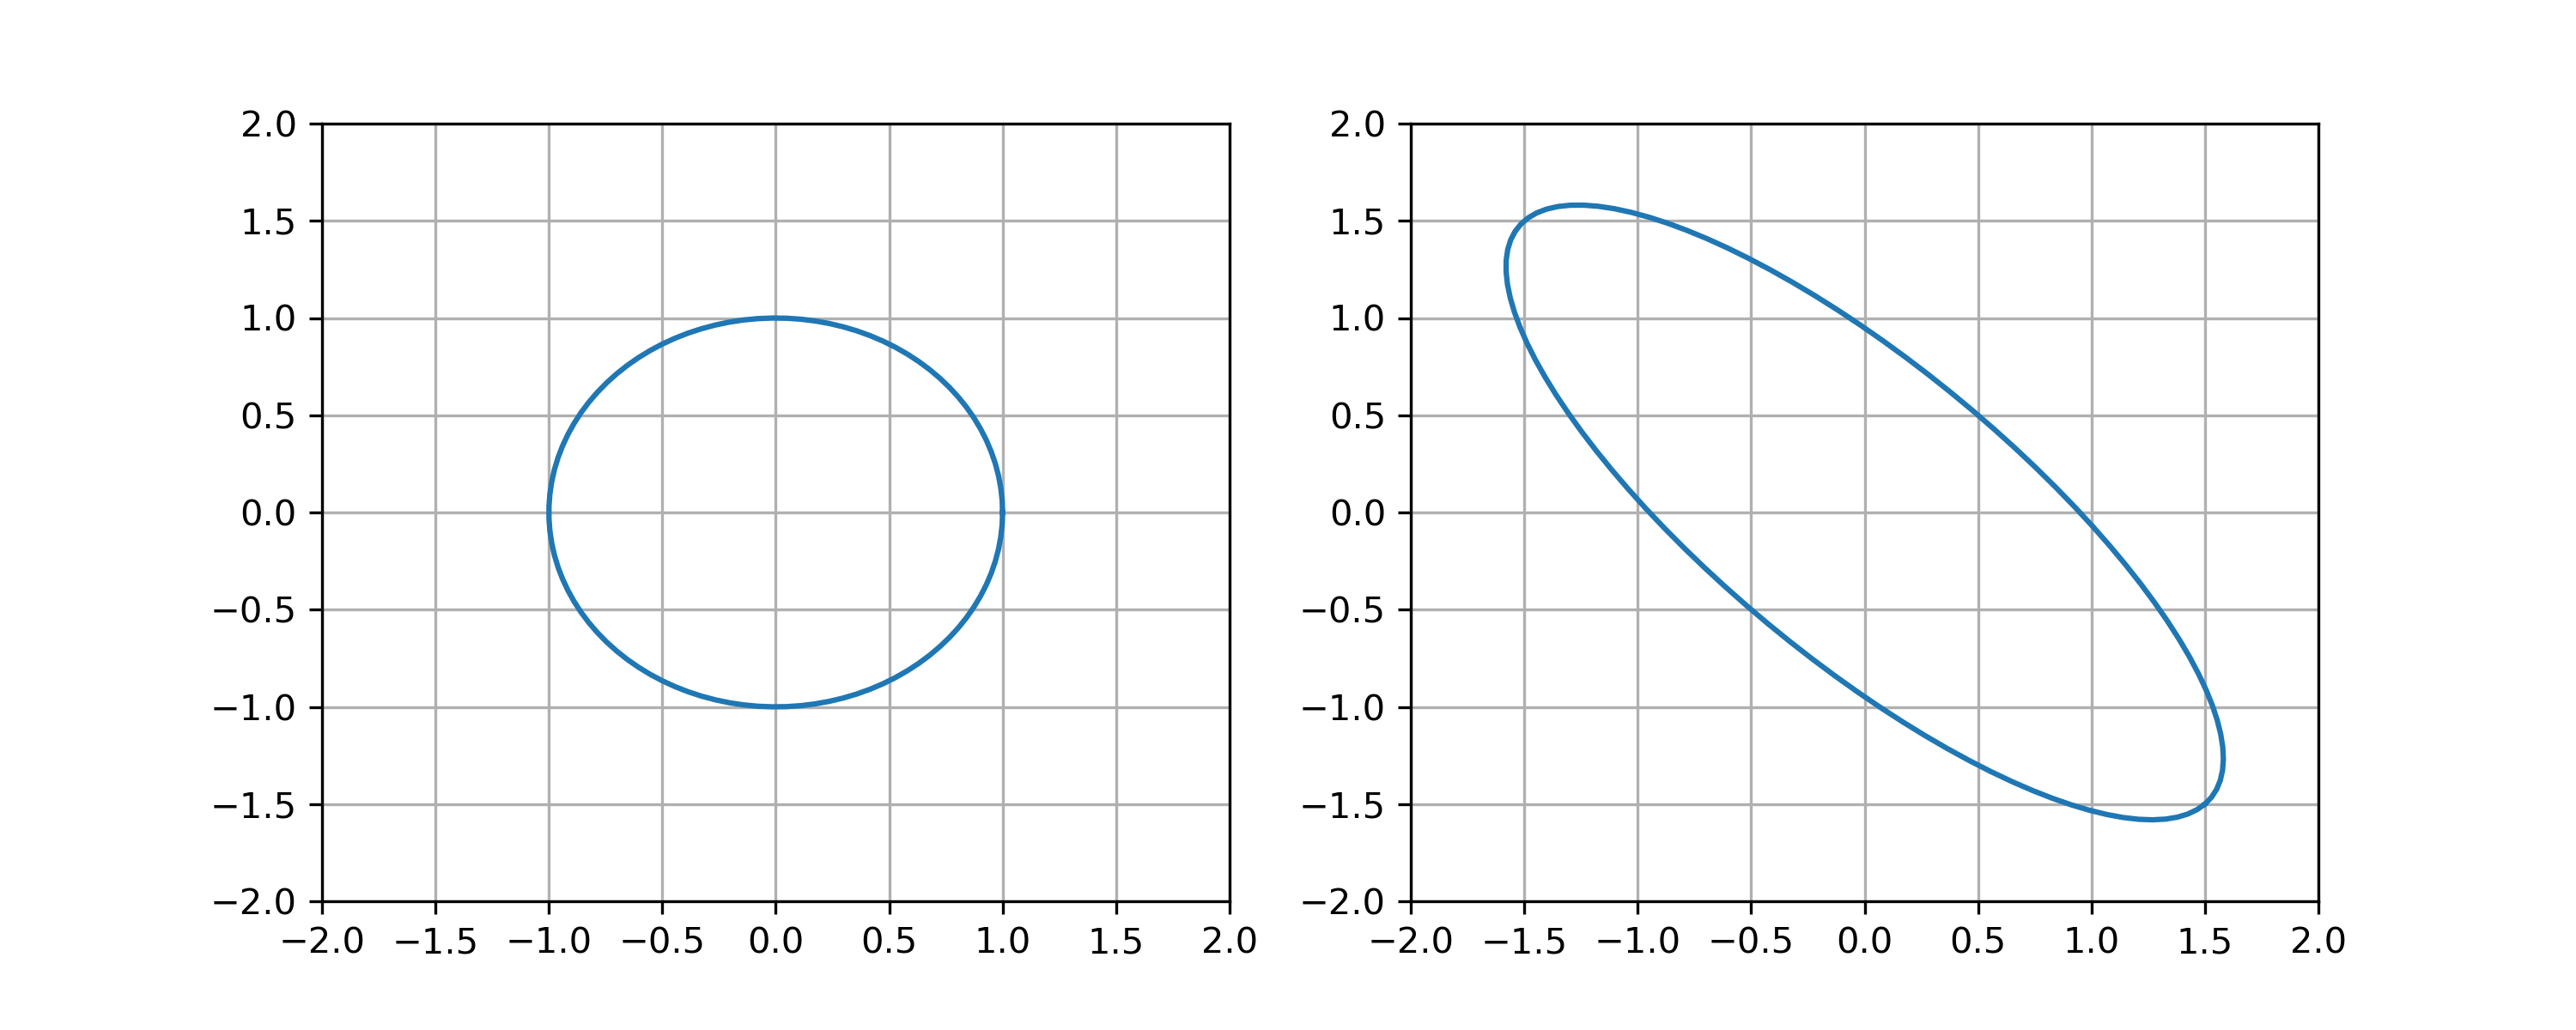
\includegraphics[width=6in]{img01.png}
\end{center}
Observe the maximum stretch of a unit vector is $\| A \| =  3\sqrt{2}/2$, the minimum stretch $\| A^{-1} \| = \sqrt{2}/2$ and the condition number is $\mathrm{cond}(A) = 3$.
\end{example}

\begin{proposition}
Let $A$ be a nonsingular matrix and consider the linear system $A \bs{x} = \bs{b}$. If a small change $\Delta \bs{b}$ corresponds to a change $\Delta \bs{x}$ in the sense that $A(\bs{x} + \Delta \bs{x}) = \bs{b} + \Delta \bs{b}$, then
$$
\frac{\| \Delta \bs{x} \|}{\| \bs{x} \|} \leq \mathrm{cond}(A) \frac{\| \Delta \bs{b} \|}{\| \bs{b} \|}
$$
See  \cite[p.58]{MH}.

\begin{proof}
Since $A \bs{x} = \bs{b}$, we have $\Delta x = A^{-1} \Delta \bs{b}$. Computing norms we find
\begin{align*}
\| \bs{b} \| &= \| A \bs{x} \| \\
\| \Delta \bs{x} \| \| \bs{b} \| &= \| A^{-1} \Delta \bs{b} \| \| A \bs{x} \| \\
\| \Delta \bs{x} \| \| \bs{b} \| &\leq \| A^{-1} \| \| \Delta\bs{b} \| \| A \| \| \bs{x} \| \\
\frac{\| \Delta \bs{x} \|}{ \| \bs{x} \|}  &\leq  \| A \| \| A^{-1} \| \frac{\| \Delta \bs{b} \|}{\| \bs{b} \|}
\end{align*}
\end{proof}
\end{proposition}

\begin{definition}
Given a vector $\bs{b}$ and small perturbation $\Delta \bs{b}$, the {\bf relative change} (or {\bf relative error}) is
$$
\frac{\| \Delta \bs{b} \|}{\| \bs{b} \|}
$$
\end{definition}

\begin{note}
The error bound
$$
\frac{\| \Delta \bs{x} \|}{\| \bs{x} \|} \leq \mathrm{cond}(A) \frac{\| \Delta \bs{b} \|}{\| \bs{b} \|}
$$
implies that if $A$ has a large condition number, then small changes in $\bs{b}$ may result in {\it very} large changes in the solution $\bs{x}$. In other words, the solution is sensitive to errors and is {}.
\end{note}